\scanpage{47}
\mspage{3)}
which form a groupoid $\deleted{\mathrm{MD}}.\ \mathrm{Grbip}$
or $(\unsure{\mathrm{Grabipond}})$

Objects : \inserted{finite} graphs $(S,\vec A,\sigma,o)$
\inserted{$+$ additional structures},
(which may have isolated vertices, closed loops, a fortiori
several edges between two vertices, and also ``\uline{free edges}''
\inserted{(``vertices'', ``\unsure{holes|arcs}'')}
corresponding to the fixed points of $\sigma$)
$S,\vec A$ finite sets, $\sigma:\vec A\longrightarrow\vec A$ involution,
$o:\vec A\longrightarrow S$ map ``origin''.
One is given in addition
\diagram{\begin{tikzcd}[ampersand replacement=\&]
S\arrow[r,"\deleted{\unsure{g}}\inserted{\unsure{\gamma}}"]\&
\mathbb N
\end{tikzcd}}
(map ``genus'' or ``weight'')

\diagram{\begin{tikzcd}[ampersand replacement=\&]
\deleted{\unsure{\widetilde A}}=\unsure{A_\ell}
\arrow[r,"r\deleted{\unsure{\rho_2}}"]\&\mathbb N
\end{tikzcd}}
(map \deleted{\unsure{rigidification}}
``rigidification index'')

\deleted{$\unsure{A_\ell}\quad\text{``\unsure{free edges}''}$}
$\underset{\mathrm{def}}{\unsure{A_\ell}\subset\vec A/\sigma}$
\deleted{``\unsure{set of additional vertices}''}

\margin{not precise enough as a datum. The weighting of an edge must be
replaced by that of a combinatorial polygon
$\unsure{T_a}$ with $\omega(\unsure{T_a})\simeq\omega(a)$.}
\margin{I have indicated a weighting of the vertices, but not of the edges}

\figure{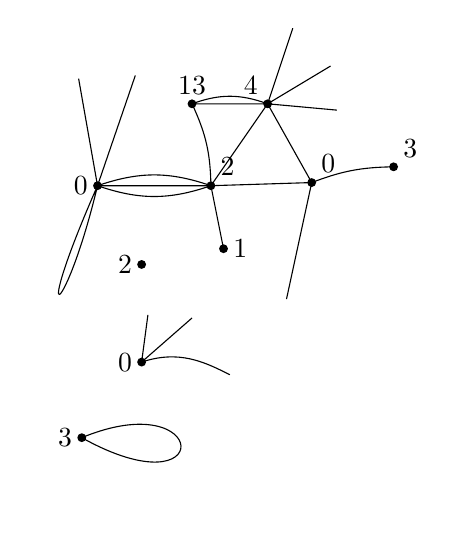
\begin{tikzpicture}[scale=.8]
\coordinate (a) at (0,0); \coordinate (b) at (1.8,0);
\coordinate (c) at (3.4,.05); \coordinate (d) at (2.7,1.3);
\coordinate (e) at (1.5,1.3); \coordinate (f) at (2,-1);
\coordinate (g) at (4.7,.3);
\draw (a)--(b)--(c)--(d)--(b)--(f);
\draw (a) to[bend left=19] (b) (a) to[bend right=19] (b);
\draw (a) .. controls (-1.1,-2.5) and (-.5,-2.1) .. (a);
\draw (a)--(-.3,1.7) (a)--(.6,1.75);
\draw (b) to[bend right=12] (e);
\draw (e)--(d) (e) to[bend left=20] (d);
\draw (d)--(3.1,2.5) (d)--(3.7,1.9) (d)--(3.8,1.2);
\draw (c)--(3,-1.8) (c) to[bend left=10] (g);
\foreach \p/\lab/\pos in {a/0/left,b/2/above right,c/0/above right,d/4/above left,e/13/above,f/1/right,g/3/above right}
{\fill (\p) circle(2pt); \node[\pos] at (\p) {$\lab$};}
\fill (.7,-1.25) circle(2pt); \node[left] at (.7,-1.25) {$2$};
\fill (.7,-2.8) circle(2pt); \node[left] at (.7,-2.8) {$0$};
\draw (.7,-2.8)--(.8,-2.05) (.7,-2.8)--(1.5,-2.1)
(.7,-2.8)..controls(1.3,-2.6)and(1.7,-2.8)..(2.1,-3);
\fill (-.25,-4) circle(2pt); \node[left] at (-.25,-4) {$3$};
\draw (-.25,-4).. controls(1.8,-3.15)and(1.9,-5.2)..(-.25,-4);
\end{tikzpicture}}

\deleted{Or again, put $\widetilde S=S\amalg A_\ell$, identified
with the set of all the ``vertices'', \deleted{\unsure{marked}} and
``\uline{marked}'' (that is $\in S$) and ``\unsure{free}''
\inserted{(that is corresponding to $\alpha\in A_\ell$)}
of the graph, one gives
\diagram{\begin{tikzcd}[ampersand replacement=\&]
\widetilde S\arrow[r,"\pi"]\&\mathbb N
\end{tikzcd}}
(\uline{weighting} of the graph)}

\margin{\[
\widetilde S=S\amalg\deleted{\unsure{S_\ell}}\inserted{A_\ell}
\qquad\deleted{\unsure{\mathrm{apparent}}}
\]
\[
\widetilde A=\vec A/\sigma=A\amalg A_\ell.
\]
\diagram{\begin{tikzcd}[ampersand replacement=\&,column sep=small]
\vec A\arrow[d] = \&\underbrace{\vec A_0}_{\vec A\setminus\vec A^\sigma}
\arrow[d,"\deg2"]\amalg\&
\underbrace{\vec A_\ell}_{\vec A^\sigma}\arrow[d,"\deg1"]\\
\widetilde A = \&A\amalg\&A_\ell
\end{tikzcd}}
Order of a vertex
\[
\sigma(s)=\underbrace{\sigma_\ell(s)}_{\substack{\text{corresponds to the ``holes''}\\
\text{or gluing circles}}}+\sigma_0(s)
\]}

The datum of the \uline{graph} underlying a
$\deleted{\mathrm{MD}}\inserted{\mathrm{bip.}}$ graph amounts to that of a corresponding
``ordinary'' graph (without free edges that is where $\sigma$ acts
without fixed points), that is
\[
\left(S,(\vec A\setminus\vec A^\sigma),
 \sigma|(\vec A\setminus\vec A^\sigma),
 o|(\vec A\setminus\vec A^\sigma)\right),
\]
\uline{plus} a \inserted{finite} set $A_\ell$
(free \uline{edges})
\deleted{or ``hole-vertices'')} and a map
\diagram{\begin{tikzcd}[ampersand replacement=\&]A_\ell\arrow[r]\&S\end{tikzcd}}

\uline{Arrows} The isomorphisms of such structures
\mspage{46}
